\section{Hello World ROM Hacking!}
\subsection{Conceptos}
\begin{frame}[fragile]{Números hexadecimales}
    \begin{uncoverenv}<2->Decimal: 0 1 2 3 4 5 6 7 8 9
    \begin{lstlisting}
    0 1 2 3 4 5 6 7 8 9 10 11 12 13 ...\end{lstlisting}\end{uncoverenv}

    \begin{uncoverenv}<3->Binario: 0 1
    \begin{lstlisting}
    0 1 10 11 100 101 110 111 1000 ...
    0 1  2  3   4   5   6   7    8\end{lstlisting}\end{uncoverenv}

    \begin{uncoverenv}<4->Octal: 0 1 2 3 4 5 6 7
    \begin{lstlisting}
    0 1 2 3 4 5 6 7 10 11 12 13 14 ...
    0 1 2 3 4 5 6 7  8  9 10 11 12\end{lstlisting}\end{uncoverenv}

    \begin{uncoverenv}<5->Hexadecimal: 0 1 2 3 4 5 6 7 8 9 A B C D E F
    \begin{lstlisting}
    0 1 2 3 4 5 6 7 8 9  A  B  C  D  E  F 10 11 12 ...
    0 1 2 3 4 5 6 7 8 9 10 11 12 13 14 15 16 17 18\end{lstlisting}\end{uncoverenv}
\end{frame}

\begin{frame}{Números hexadecimales}
    \begin{itemize}
        \item<1-> Prefijo: \texttt{0x} -> \texttt{0xA, 0xFB, 0xCA, 0xFE}

        \item<2-> Representación de tipos:
        \begin{itemize}
            \footnotesize
            \item<3-> 1: \texttt{[0, 15] 0xC (12)} -> \textonehalf~byte, 4 bits
            \item<4-> 2: \texttt{[0, 255] 0xC0 (192)} -> 1 byte, 8 bits
            \item<5-> 4: \texttt{[0, 65,535] 0x0200 (512)} -> 2 bytes, 16 bits, ushort, WORD
            \item<6-> 8: \texttt{[0, 4,294,967,295] 0xB7000000 (3,070,230,528)} -> \\ 4 bytes, 32 bits, uint, DWORD
        \end{itemize}
        \normalsize

        \item<7-> Operaciones a nivel de bits:
        \begin{itemize}
            \footnotesize
            \item<9-> Filtrar/Máscaras: \texttt{0xAFC2 AND 0xF800 = 0xA800}
            \item<10-> Formar valores: \texttt{0xB7000000 OR 0xCADB00 = 0xB70ADB00}
            \item<11-> Cifrar: \texttt{0xCAFE XOR 0xAAAA = 0x6054, NOT 0xBEBE = 0x3501}
            \item<12-> Desplazamientos: \texttt{0xC2 << 4 = 0xC20, 0xA800 >> 8 = 0xA8}
        \end{itemize}
    \end{itemize}
    \visible<8->{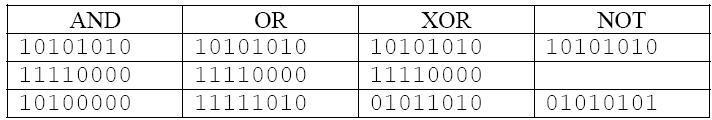
\includegraphics[width=\textwidth]{bitop.png}}
\end{frame}


\begin{frame}{Endianness}
    \begin{block}{}
        Orden en el que se guardan los bytes que forman valores mayores a 8 bits (ushort, uint, ulong, \ldots). MSB \textrightarrow LSB.
    \end{block}
    \centering{}Big Endian:
    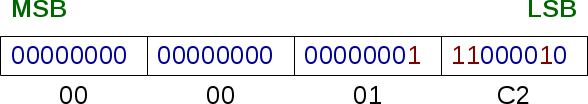
\includegraphics[width=0.9\textwidth]{big_endian.png}
    \vfill
    Little Endian (más común):
    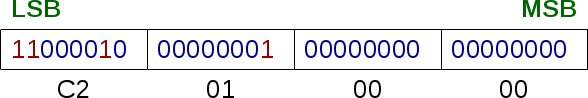
\includegraphics[width=0.9\textwidth]{little_endian.png}
\end{frame}

\subsection{Investigando un juego}
\begin{frame}{Especificación de juegos de NDS}
\end{frame}

\begin{frame}{Cabecera de los juegos}
\end{frame}

\begin{frame}{Buscar los textos en hexadecimal}
\end{frame}

\begin{frame}{Tinke}
    % Abrir tinke, acciones típicas y significado de iconos
\end{frame}

\begin{frame}{Tinke}
    % Buscar texto desde Tinke
\end{frame}

\subsection{Editar juegos}
\begin{frame}{Modificando texto}
    % Juego: Layton
    % Extraer archivo
    % Editarlo con Notepad++ o Atom
    % Importar archivo
    % Generar ROM
    % Probar en DeSmuME
\end{frame}

\subsection{Distribuyamos los cambios}
\begin{frame}{Legalidad}
\end{frame}

\begin{frame}{Parches}
\end{frame}

\begin{frame}{xDelta}
\end{frame}
